\documentclass[fullscreen=true]{beamer}
\usepackage[utf8]{inputenc}
\usepackage[english,russian]{babel}
\usepackage{amssymb,amsfonts,amsmath,mathtext}
\usepackage{enumerate,indentfirst,tikz,pgf}
\usetikzlibrary{mindmap,trees}
\usetikzlibrary{shadows}

\usetheme{Warsaw}

\usecolortheme{default}

\setbeamertemplate{background canvas} [vertical
shading][bottom=blue!20,top=blue!60]

\setbeamertemplate{blocks}[rounded][shadow=true]

%\usecolortheme{seahorse}
\usefonttheme{professionalfonts}


% ----------- Дополнительные спецификации ----------
\newcounter{tasknum}
\newcommand{\task}{\addtocounter{tasknum}{1}
\arabic{tasknum}}
%---------------------------------------------------

\begin{document}

% ---------- Титульный слайд -------------
\title{Статистический анализ данных. Спецкурс.}
\author{Ботанический сад-институт ДВО РАН}% \\ \texttt{kisl\_di@mail.ru}}
\date{Кислов Д.Е. \\ 05 сентября 2016 г}
\maketitle
% -----------------------------------------


%---------------- слайд 2 -----------------
\begin{frame}
\frametitle{Структура и задачи курса}
\begin{itemize}
\item формирование общих представлений о методах теории вероятностей и
математической статистики;
\item знакомство с математическими методами статистики;
\item изучение многофункциональных программных сред для решения практических
задач;
\item \ldots
\end{itemize}
\end{frame}
% -----------------------------------------

%---------------- слайд 3 -----------------
\begin{frame}
\frametitle{Важные исторические даты}

\begin{itemize}

\item[$\blacklozenge$] Формирование понятия случайного
явления;\newline
        \begin{itemize}
        \item Древнегреческие философы (Гераклит, Демокрит и др.)
       % \item Августин блаженный (около 400 г.): "...это
       % делается силою случая, всегда и всюду действующего в природе";
        \item Боэций С. (Рим, ок. 520 г):  \newline
        "случайность --- не подлинное явление, а результат скрещения независимых друг
        от друга процессов, каждый из которых имеет вполне определенную
        причину";
        \end{itemize}

\item[$\blacklozenge$] Предпосылки возникновения теории вероятностей (X-XI век);

\item[$\blacklozenge$] Попытки систематического изложения теории
                    (Д. Кардано (1501-1576), Н. Тарталья (1499--1557));
\end{itemize}
\end{frame}

% -----------------------------------------

%---------------- слайд 4 -----------------
\begin{frame}
\frametitle{Важные исторические даты}
\begin{itemize}
\item[$\blacklozenge$] Х.~Гюйгенс (1629--1695): Первая книга по
теории вероятностей -- "О расчетах в азартной игре".  Введено
понятие среднего значения --- математического ожидания;
\item[$\blacklozenge$] Зарождение статистики: Джон Граунт
(1620--1674); Вильям Петти (1623--1687). "Естественные и
политические наблюдения над бюллетенями смертности" (Граунт, 1662),
"Политическая арифметика" (Петти, 1676);
\end{itemize}
\begin{columns}
\begin{column}{4cm}
\begin{figure}
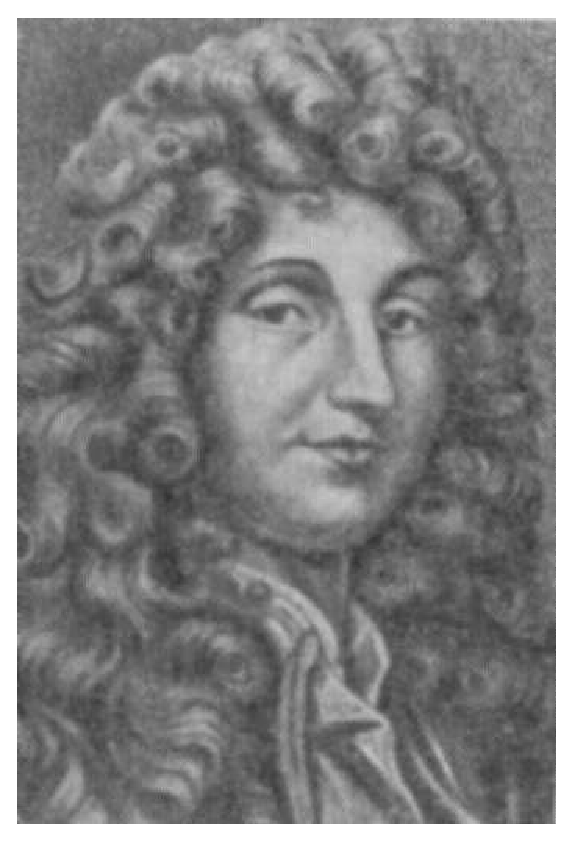
\includegraphics[height=3cm]{gugens}
\caption{Х. Гюйгенс}
\end{figure}
\end{column}
\begin{column}{4cm}
\begin{figure}
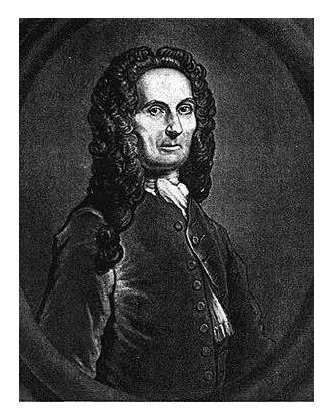
\includegraphics[height=3cm]{moivre}
\caption{А. Муавр}
\end{figure}
\end{column}
\begin{column}{4cm}
\begin{figure}
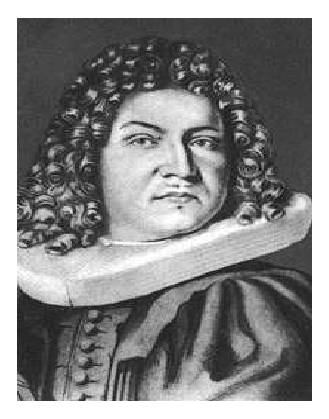
\includegraphics[height=3cm]{bernulli}
\caption{Я. Бернулли}
\end{figure}
\end{column}
\end{columns}
\end{frame}
% -----------------------------------------


%---------------- слайд 5 -----------------
\begin{frame}
\frametitle{Важные исторические даты}
\begin{itemize}
\item[$\blacklozenge$] И. Ньютон (1642--1727) --- Я. Бернулли
(1654--1705); "Искусство предположений" (Бернулли, 1713);

\item[$\blacklozenge$] Абрахам де Муавр (1667--1754): "Учение о
случаях" (Муавр, 1733); П.С. Лаплас (1749 -- 1827);

\item[$\blacklozenge$] Т. Байес (1702--1761) "Формула Байеса"
(Байес, 1763);

\item[$\blacklozenge$] Теория ошибок (конец XVIII) --- К.Ф. Гаусс (1777-1855);

\item[$\blacklozenge$] А.Н. Колмогоров (1903--1987) --- Аксиоматизация
теории вероятностей (Колмогоров, 1933);

\item[$\blacklozenge$] К.~Пирсон (1857--1936) --- Критерий $\chi^2$;
Р.А.~Фишер (1890--1962) --- метод максимального правдоподобия;
E.~Нейман (1894--1977)  --- статистическая
проверка гипотез;
\end{itemize}
\end{frame}
% -----------------------------------------




\end{document}